\chapter{ANALISIS DAN PERANCANGAN SISTEM}
\par Bab ini menjelaskan analisis dan perancangan sistem untuk mencapai tujuan dari tugas akhir, meliputi perancangan data, proses, dan analisa implementasi secara umum.

\section{Analisis Sistem}
\par Subbab ini akan membahas mengenai hasil analisa perangkat lunak push notification terpusat.
Analisis yang dilakukan meliputi analisis permasalahan, deskripsi umum sistem, dan spesifikasi kebutuhan perangkat lunak.

\subsection{Analisis Permasalahan}
\par Permasalahan yang diangkat pada tugas akhir ini adalah keandalan aplikasi push notification terpusat untuk mengirimkan notifikasi ke perangkat pengguna dalam jumlah besar. Berdasarkan hasil pengujian yang dilakukan oleh pengembang sebelumnya, tingkat keberhasilan pengiriman notifikasi ke 3000 pengguna hanya sebesar 63,8 persen \cite{application-thesis}.
\par Arsitektur \textit{message queue} pada aplikasi push notification terpusat dapat dilihat pada Gambar \ref{arsitektur_message_queue_lama}. Terdapat beberapa \textit{thread} yang menambahkan dan mengambil pesan dari antrian secara bersamaan. Berdasarkan analisis yang penulis lakukan, struktur data \textit{linked list} yang digunakan oleh antrian tidak mendukung perubahan data secara bersamaan \cite{linkedlist-online}. Konsekuensinya, pesan yang berada di antrian bisa saja hilang tanpa ada \textit{error} yang terdeteksi oleh aplikasi. Potongan kode implementasi \textit{message queue} dapat dilihat pada \nameref{lampiran:queue_service}.
\begin{figure}[H]
	\centering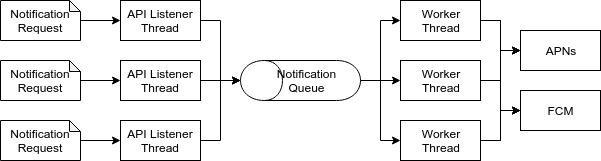
\includegraphics[width=1\textwidth]{bab3/figures/arsitektur_message_queue_lama.jpg}
	\caption{Arsitektur \textit{Message Queue} Lama}
	\label{arsitektur_message_queue_lama}
\end{figure}

\subsection{Deskripsi Umum Sistem}
\par Aplikasi push notification terpusat merupakan layanan yang digunakan untuk mengirim \textit{push notification} ke perangkat pengguna secara terjadwal dan \textit{asynchronous}. Pada tugas akhir ini akan dibagi menjadi 3 modul, yaitu Scheduler, Sender APN, dan Sender FCM.
\par Secara umum, Scheduler bertanggung jawab untuk penjadwalan pengiriman notifikasi, Sender APN bertanggung jawab untuk mengirimkan notifikasi yang diantrikan ke perangkat iOS lewat layanan APNs, dan Sender FCM bertanggung jawab untuk mengirimkan notifikasi yang diantrikan ke perangkat Android dan Web lewat layanan FCM.
\par Komunikasi antar modul aplikasi push notification terpusat menggunakan metode \textit{message queue} dengan pola \textit{publish/subscribe}, dan antrian yang dibagi berdasarkan topik. Topik antrian ditentukan berdasarkan tipe perangkat penerima notifikasi, yaitu Android, Web, atau iOS.
\par Pada tugas akhir ini, komunikasi antar modul dan penyimpanan antrian akan menggunakan \textit{Kafka}, sistem basis data akan menggunakan \textit{SQL Server}, dan implementasi modul-modul aplikasi akan menggunakan bahasa pemrograman \textit{Java} dengan kerangka kerja \textit{Spring}.

\subsection{Spesifikasi Kebutuhan Perangkat Lunak}
\par Subbab ini membahas spesifikasi kebutuhan perangkat lunak dari hasil analisis yang telah dilakukan. Subbab ini berisi kebutuhan perangkat lunak yang direpresentasikan dalam bentuk kebutuhan fungsional, kebutuhan non fungsional, dan diagram kasus penggunaan.

\subsubsection{Aktor}
\begin{longtable}{|p{2cm}|p{7cm}|}
    \hline
    \textbf{Aktor} & \textbf{Tugas} \\ \hline
    Scheduler & Membuat dan menjadwalkan pengiriman \textit{packet} notifikasi. \\ \hline
    Sender APN & Mengirimkan \textit{packet} notifikasi untuk perangkat iOS. \\ \hline
    Sender FCM & Mengirimkan \textit{packet} notifikasi untuk perangkat Android dan Web. \\ \hline
    \caption{Aktor pada sistem}
\end{longtable}

\subsubsection{Kebutuhan Fungsional}
\begin{longtable}{|p{0.6cm}|p{3cm}|p{5cm}|}
    \hline
    \textbf{No.} & \textbf{Kebutuhan Fungsional} & \textbf{Deskripsi} \\ \hline
    F01 & Pembuatan Packet & Jika terdapat batch yang belum dan boleh dibuatkan packet, sistem dapat membuatkan packet dari batch tersebut. \\ \hline
    F02 & Menambahkan Packet ke Antrian & Jika terdapat packet yang belum dan sudah waktunya dikirim, sistem dapat menambahkan packet tersebut ke antrian pengiriman. \\ \hline
    F03 & Pengiriman Packet ke APNs & Jika terdapat packet untuk perangkat iOS di antrian pengiriman, sistem dapat mengambil packet dari antrian dan mengirim packet ke layanan APNs. \\ \hline
    F04 & Pengiriman Packet ke FCM & Jika terdapat packet untuk perangkat Android dan Web di antrian pengiriman, sistem dapat mengambil packet dari antrian dan mengirim packet ke layanan FCM. \\ \hline
    F05 & Menampilkan Penggunaan Sumber Daya & Jika mendapat request HTTP tertentu, sistem dapat menampilkan penggunaan sumber daya (CPU dan Memori) yang digunakan dalam bentuk response HTTP. \\ \hline
    F06 & Menampilkan Status Kesehatan & Jika mendapat request HTTP tertentu, sistem dapat menampilkan kondisi layanan yang berhubungan dengan sistem (Kafka dan SQL Server) dalam bentuk response HTTP. \\ \hline
    F07 & Menampilkan Konfigurasi & Jika mendapat request HTTP tertentu, sistem dapat menampilkan konfigurasi aplikasi sistem dalam bentuk response HTTP. \\ \hline
    F08 & Menampilkan Log & Jika mendapat request HTTP tertentu, sistem dapat menampilkan isi log sistem dalam bentuk response HTTP. \\ \hline
    \caption{Kebutuhan fungsional sistem}
\end{longtable}

\subsubsection{Kebutuhan Non Fungsional}
\begin{longtable}{|p{0.6cm}|p{2cm}|p{5.5cm}|}
    \hline
    \textbf{No.} & \textbf{Parameter} & \textbf{Deskripsi} \\ \hline
    1 & Reliability & Aplikasi dapat mengirimkan 1 juta notifikasi ke layanan FCM \& APNs dengan tingkat sempurna. \\ \hline
    2 & Availability & Aplikasi dapat menangani pengiriman 1 juta notifikasi tanpa \textit{down}. \\ \hline
    \caption{Kebutuhan non fungsional sistem}
\end{longtable}

\subsubsection{Diagram Kasus Penggunaan}
\par Subbab ini menjelaskan kasus penggunaan perangkat lunak secara rinci. Kasus penggunaan dibuat berdasarkan hasil analisis yang pada subbab sebelumnya.
\par Diagram kasus penggunaan untuk setiap modul (Scheduler, Sender APN, dan Sender FCM) aplikasi \textit{push notification} terpusat dapat dilihat pada gambar~\ref{diagram_kasus_penggunaan}.
\begin{figure}[H]
    \centering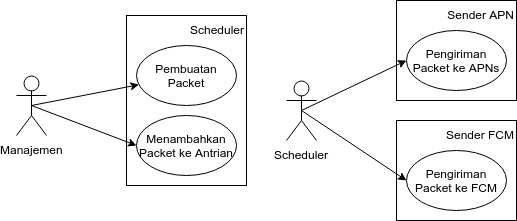
\includegraphics[width=1\textwidth]{bab3/figures/diagram_kasus_penggunaan.jpg}
    \caption{Diagram Kasus Penggunaan}
    \label{diagram_kasus_penggunaan}
\end{figure}

% template tabel deskripsi kasus penggunaan
\newcommand\tableUcDesc[8] {
\begin{longtable}{|p{2.5cm}|p{6.5cm}|}
    \hline
    \textbf{Komponen} & \textbf{Deskripsi} \\ \hline
    Kode & #1 \\ \hline
    Nama & #2 \\ \hline
    Aktor & #3 \\ \hline
    Kondisi Awal & #4 \\ \hline
    Kondisi Akhir & #5 \\ \hline
    Alur Normal & #6 \\ \hline
    Alur Alternatif & #7 \\ \hline
    \caption{Kasus Penggunaan #2}
\end{longtable}
}

\paragraph{Pembuatan Packet}
\par Pada kasus ini, Scheduler akan mencari batch yang belum dan boleh dibuatkan \textit{packet} secara berkala. Jika ada, Scheduler akan membuatkan \textit{packet} untuk \textit{batch} tersebut.
\tableUcDesc
{UC01}
{Pembuatan Packet}
{Scheduler}
{Terdapat batch yang belum dan boleh dibuatkan packet}
{Packet dibuat untuk batch tersebut}
{
\begin{enumerate}
    \item Aktor memeriksa apakah terdapat batch yang belum dan boleh dibuatkan packet.
    \item Aktor membuatkan data packet dari batch tersebut.
    \item Aktor menyimpan data packet dan memperbarui data batch.
\end{enumerate}
}
{-}

\paragraph{Menambahkan Packet ke Antrian}
\par Pada kasus ini, Scheduler akan mencari \textit{packet} yang belum dan sudah waktunya dikirim secara berkala. Jika ada, Scheduler akan menambahkan \textit{packet} tersebut ke antrian \textit{Kafka} dengan topik yang dibagi berdasarkan jenis perangkat penerima.
\tableUcDesc
{UC02}
{Menambahkan Packet ke Antrian}
{Scheduler}
{Terdapat packet yang belum dan sudah waktunya dikirim}
{Packet ditambahkan ke antrian}
{
\begin{enumerate}
    \item Aktor memeriksa apakah terdapat packet yang belum dan sudah waktunya dikirim.
    \item Aktor menambahkan packet ke dalam antrian dengan spesifikasi topik sebagai berikut:
    \begin{enumerate}
        \item Topik "android" untuk packet dengan target perangkat Android.
        \item Topik "web" untuk packet dengan target perangkat Web.
        \item Topik "ios" untuk packet dengan target perangkat iOS.
    \end{enumerate}
    \item Aktor memperbarui data packet (status sedang menunggu).
\end{enumerate}
}
{-}

\paragraph{Pengiriman Packet ke APNs}
\par Pada kasus ini, Sender APN akan menunggu \textit{Kafka} mengirimkan packet yang ada di antrian topik "ios". Setelah packet diterima, packet akan dikirimkan ke layanan APNs.
\tableUcDesc
{UC03}
{Pengiriman Packet ke APNs}
{Sender APN}
{Terdapat packet di antrian topik "ios"}
{Packet diterima oleh layanan APNs}
{
\begin{enumerate}
    \item Aktor menerima packet dari antrian topik "ios".
    \item Aktor mengirimkan request notifikasi ke layanan APNs berdasarkan data packet.
    \item Aktor memperbarui data packet berdasarkan response dari APNs (berhasil atau gagal dan alasan gagal).
\end{enumerate}
}
{-}

\paragraph{Pengiriman Packet ke FCM}
\par Pada kasus ini, Sender FCM akan menunggu \textit{Kafka} mengirimkan packet yang ada di antrian topik "android" dan "web". Setelah packet diterima, packet akan dikirimkan ke layanan FCM.
\tableUcDesc
{UC04}
{Pengiriman Packet ke FCM}
{Sender FCM}
{Terdapat packet di antrian topik "android" atau "web"}
{Packet diterima oleh layanan FCM}
{
\begin{enumerate}
    \item Aktor menerima packet dari antrian topik "android" atau "web".
    \item Aktor mengirimkan request notifikasi ke layanan FCM berdasarkan data packet.
    \item Aktor memperbarui data packet berdasarkan response dari FCM (berhasil atau gagal dan alasan gagal).
\end{enumerate}
}
{-}

\paragraph{Menampilkan Penggunaan Sumber Daya}
\par Pada kasus ini, Scheduler, Sender APN, dan Sender FCM dapat menampilkan penggunaan sumber daya (CPU dan Memori) yang digunakan aplikasi dengan menggunakan REST API.
\tableUcDesc
{UC05}
{Menampilkan Penggunaan Sumber Daya}
{Scheduler, Sender APN, Sender FCM}
{Aktor menerima request HTTP}
{Aktor mengembalikan response HTTP}
{
	\begin{enumerate}
		\item Aktor menerima request HTTP untuk melihat penggunaan sumber daya.
		\item Aktor memeriksa metrik penggunaan sumber daya dari sistem operasi.
		\item Aktor mengembalikan hasil pemeriksaan penggunaan sumber daya dalam bentuk response HTTP.
	\end{enumerate}
}
{-}

\paragraph{Menampilkan Status Kesehatan}
\par Pada kasus ini, Scheduler, Sender APN, dan Sender FCM dapat menampilkan status kesehatan aplikasi dan layanan yang terhubung dengan aplikasi dengan menggunakan REST API.
\tableUcDesc
{UC06}
{Menampilkan Status Kesehatan}
{Scheduler, Sender APN, Sender FCM}
{Aktor menerima request HTTP}
{Aktor mengembalikan response HTTP}
{
	\begin{enumerate}
		\item Aktor menerima request HTTP untuk melihat status kesehatan.
		\item Aktor memeriksa apakah aktor dapat terhubung ke layanan-layanan yang dibutuhkan oleh aktor untuk beroperasi.
		\item Aktor mengembalikan status (bisa diakses atau tidak) layanan-layanan yang dibutuhkan dalam bentuk response HTTP.
	\end{enumerate}
}
{-}

\paragraph{Menampilkan Konfigurasi}
\par Pada kasus ini, Scheduler, Sender APN, dan Sender FCM dapat menampilkan konfigurasi aplikasi dengan menggunakan REST API.
\tableUcDesc
{UC07}
{Menampilkan Konfigurasi}
{Scheduler, Sender APN, Sender FCM}
{Aktor menerima request HTTP}
{Aktor mengembalikan response HTTP}
{
	\begin{enumerate}
		\item Aktor menerima request HTTP untuk melihat konfigurasi aplikasi.
		\item Aktor memeriksa konfigurasi \textit{Spring} yang ada di aplikasi.
		\item Aktor memeriksa \textit{environment variable} yang ada di sistem operasi.
		\item Aktor mengembalikan konfigurasi \textit{Spring} dan \textit{environment variable} yang ada dalam bentuk response HTTP.
	\end{enumerate}
}
{-}

\paragraph{Menampilkan Log}
\par Pada kasus ini, Scheduler, Sender APN, dan Sender FCM dapat menampilkan \textit{log} yang dikeluarkan oleh aplikasi dengan menggunakan REST API.
\tableUcDesc
{UC08}
{Menampilkan Log}
{Scheduler, Sender APN, Sender FCM}
{Aktor menerima request HTTP}
{Aktor mengembalikan response HTTP}
{
\begin{enumerate}
	\item Aktor menerima request HTTP untuk melihat log aplikasi.
	\item Aktor mencari lokasi file log yang digunakan aplikasi untuk menyimpan log.
	\item Aktor mengembalikan isi file log dalam bentuk response HTTP.
\end{enumerate}
}
{-}

\section{Perancangan Sistem}
\par Subbab ini akan membahas tahapan perancangan sistem yang dibagi menjadi beberapa bagian, yaitu perancangan
arsitektur, data, dan proses.

\subsection{Perancangan Arsitektur}
\par Aplikasi \textit{push notification} terpusat akan dibagi menjadi 3 modul, yaitu Scheduler,
Sender APN, dan Sender FCM.
Aplikasi dibangun dengan bahasa pemrograman Java, dengan kerangka kerja
Spring.
Aplikasi saling terhubung lewat Kafka dan SQL Server.
Secara garis besar, aplikasi ini memiliki rancangan
arsitektur pengiriman notifikasi yang dapat dilihat pada gambar~\ref{arsitektur_pengiriman_notifikasi}.
\begin{figure}[H]
    \centering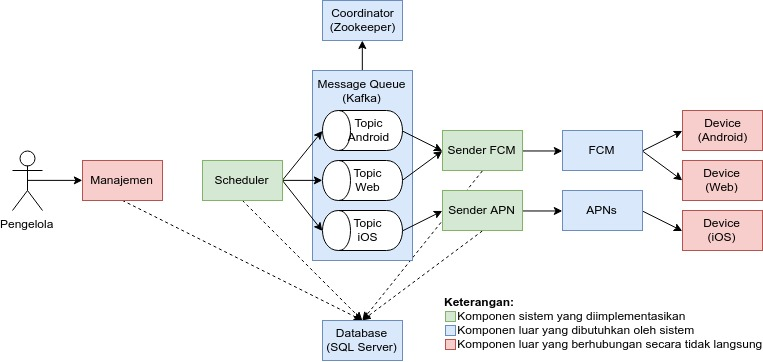
\includegraphics[width=1\textwidth]{bab3/figures/arsitektur_pengiriman_notifikasi.jpg}
    \caption{Arsitektur Pengiriman Notifikasi}
    \label{arsitektur_pengiriman_notifikasi}
\end{figure}

\subsection{Perancangan Basis Data}
\par Subbab ini membahas bagaimana rancangan basis data yang digunakan pada aplikasi \textit{push notification} terpusat. Basis data yang digunakan adalah SQL Server 2012.

\subsubsection{Tabel User}
\par Tabel user digunakan untuk menyimpan data pengguna aplikasi yang ada di Institut Teknologi Sepuluh Nopember. Rincian atribut dapat dilihat pada Tabel \ref{tabel_user}.
\begin{longtable}{|p{2cm}|p{2.5cm}|p{4.5cm}|}
    \hline
    \textbf{Atribut} & \textbf{Tipe Data} & \textbf{Deskripsi} \\ \hline
    User ID & uuid & Primary key tabel \\ \hline
    Name & varchar(150) & - \\ \hline
    Nickname & varchar(20) & - \\ \hline
    Username & varchar(255) & - \\ \hline
    Password & varchar(256) & - \\ \hline
    Email & varchar(255) & - \\ \hline
    Email Verified & numeric(1) & - \\ \hline
    Scope & varchar(4000) & - \\ \hline
    Alternate Email & varchar(255) & - \\ \hline
    Alternate Email Verified & numeric(1) & - \\ \hline
    Phone & varchar(18) & - \\ \hline
    Phone Verified & numeric(1) & - \\ \hline
    Enabled & numeric(1) & - \\ \hline
    Picture & varbinary(max) & - \\ \hline
    Gender & char(1) & - \\ \hline
    Birth Date & date & - \\ \hline
    Zone Info & varchar(40) & - \\ \hline
    Locale & varchar(10) & - \\ \hline
    Integra ID & numeric(12) & - \\ \hline
    Registration ID & varchar(25) & - \\ \hline
    Must Change Password & numeric(1) & - \\ \hline
    Sandbox & numeric(1) & - \\ \hline
    Locked & datetime & - \\ \hline
    Suspended & datetime & - \\ \hline
    Has Suspended & numeric(1) & - \\ \hline
    Group ID & int & - \\ \hline
    Auth Method ID & numeric(2) & - \\ \hline
    Created At & datetime & Tanggal dan waktu dibuat \\ \hline
    Update At & datetime & Tanggal dan waktu diperbarui \\ \hline
    \caption{Tabel User}
    \label{tabel_user}
\end{longtable}

\subsubsection{Tabel Group}
\par Tabel group digunakan untuk menyimpan data kelompok pengguna. Rincian atribut dapat dilihat pada Tabel \ref{tabel_group}.
\begin{longtable}{|p{2cm}|p{2.5cm}|p{4.5cm}|}
    \hline
    \textbf{Atribut} & \textbf{Tipe Data} & \textbf{Deskripsi} \\ \hline
    Group ID & uuid & Primary key tabel \\ \hline
    Name & varchar(100) & - \\ \hline
    Created At & datetime & Tanggal dan waktu dibuat \\ \hline
    Update At & datetime & Tanggal dan waktu diperbarui \\ \hline
    \caption{Tabel Group}
    \label{tabel_group}
\end{longtable}

\subsubsection{Tabel Group Member}
\par Tabel group member digunakan untuk menyimpan data pengguna yang menjadi anggota dari suatu kelompok. Rincian atribut dapat dilihat pada Tabel \ref{tabel_group_member}.
\begin{longtable}{|p{2cm}|p{2.5cm}|p{4.5cm}|}
    \hline
    \textbf{Atribut} & \textbf{Tipe Data} & \textbf{Deskripsi} \\ \hline
    Group ID & uuid & Grup tempat pengguna terdaftar \\ \hline
    User ID & uuid & Pengguna yang terdaftar di grup \\ \hline
    Created At & datetime & Tanggal dan waktu dibuat \\ \hline
    Update At & datetime & Tanggal dan waktu diperbarui \\ \hline
    \caption{Tabel Group Member (pn\_group\_member)}
    \label{tabel_group_member}
\end{longtable}

\subsubsection{Tabel Client}
\par Tabel client digunakan untuk menyimpan data aplikasi yang ada di Institut Teknologi Sepuluh Nopember. Rincian atribut dapat dilihat pada Tabel \ref{tabel_client}.
\begin{longtable}{|p{2cm}|p{2.5cm}|p{4.5cm}|}
    \hline
    \textbf{Atribut} & \textbf{Tipe Data} & \textbf{Deskripsi} \\ \hline
    Client ID & uuid & Primary key tabel \\ \hline
    Client Name & varchar(100) & - \\ \hline
    Client Description & varchar(250) & - \\ \hline
    Client Secret & varchar(255) & - \\ \hline
    Expires At & datetime & - \\ \hline
    Logo & varchar(100) & - \\ \hline
    Redirect URI & varchar(2000) & - \\ \hline
    Post Logout Redirect URIS & varchar(2048) & - \\ \hline
    Front Channel Logout URI & varchar(255) & - \\ \hline
    Front Channel Logout Session Required & numeric(1) & - \\ \hline
    Back Channel Logout URI & varchar(255) & - \\ \hline
    Back Channel Logout Session Required & numeric(1) & - \\ \hline
    Base URI & varchar(255) & - \\ \hline
    API Base URI & varchar(255) & - \\ \hline
    Application Type & char(1) & - \\ \hline
    Contact Name & varchar(255) & - \\ \hline
    Contact Email & varchar(255) & - \\ \hline
    Preauthorized & numeric(1) & - \\ \hline
    Grant Types & varchar(80) & - \\ \hline
    Scope & varchar(4000) & - \\ \hline
    Sandbox & numeric(1) & - \\ \hline
    Is Moderated & numeric(1) & - \\ \hline
    Visible & numeric(1) & - \\ \hline
    Category ID & int & - \\ \hline
    Auth Type ID & char(1) & - \\ \hline
    User ID & uuid & - \\ \hline
    Provider ID & uuid & - \\ \hline
    Created At & datetime & Tanggal dan waktu dibuat \\ \hline
    Update At & datetime & Tanggal dan waktu diperbarui \\ \hline
    \caption{Tabel Client}
    \label{tabel_client}
\end{longtable}

\subsubsection{Tabel Certificate}
\par Tabel certificate digunakan untuk menyimpan data sertifikat yang digunakan untuk autentikasi ke layanan APNs dan FCM. Rincian atribut dapat dilihat pada Tabel \ref{tabel_certificate}.
\begin{longtable}{|p{2cm}|p{2.5cm}|p{4.5cm}|}
    \hline
    \textbf{Atribut} & \textbf{Tipe Data} & \textbf{Deskripsi} \\ \hline
    Certificate ID & uuid & Primary key tabel \\ \hline
    Client ID & uuid & Foreign key tabel client \\ \hline
    Bundle ID & varchar(255) & Bundle ID untuk aplikasi iOS \\ \hline
    Certificate Key & text & File sertifikat yang sudah diencode dengan base64 \\ \hline
    Type & char(1) & Tipe sertifikat (FCM atau APNs) \\ \hline
    Password & varchar(255) & Kata sandi untuk sertifikat iOS \\ \hline
    \caption{Tabel Certificate}
    \label{tabel_certificate}
\end{longtable}

\subsubsection{Tabel Device}
\par Tabel device digunakan untuk menyimpan data perangkat pengguna aplikasi yang terdaftar di layanan APNs dan FCM. Rincian atribut dapat dilihat pada Tabel \ref{tabel_device}.
\begin{longtable}{|p{2cm}|p{2.5cm}|p{4.5cm}|}
    \hline
    \textbf{Atribut} & \textbf{Tipe Data} & \textbf{Deskripsi} \\ \hline
    Device ID & uuid & Primary key tabel \\ \hline
    Client ID & uuid & Client tempat perangkat terdaftar \\ \hline
    User ID & uuid & User pemilik perangkat \\ \hline
    Device Token & varchar(255) & Token yang terdaftar di layanan APNs dan FCM \\ \hline
    Device Type & char(1) & Jenis perangkat (Android, Web, atau iOS) \\ \hline
    Active & numeric(1) & Perangkat aktif atau tidak \\ \hline
    Registration Date & datetime & - \\ \hline
    Invalidate Date & datetime & - \\ \hline
    \caption{Tabel Device}
    \label{tabel_device}
\end{longtable}

\subsubsection{Tabel Batch}
\par Tabel batch digunakan untuk menyimpan data notifikasi yang akan dikirim ke beberapa perangkat. Rincian atribut dapat dilihat pada Tabel \ref{tabel_batch}.
\begin{longtable}{|p{2cm}|p{2.5cm}|p{4.5cm}|}
    \hline
    \textbf{Atribut} & \textbf{Tipe Data} & \textbf{Deskripsi} \\ \hline
    Batch ID & uuid & Primary key tabel \\ \hline
    Title & varchar(255) & Judul notifikasi \\ \hline
    Body & varchar(255) & Isi pesan notifikasi \\ \hline
    Image & varchar(255) & Nama atau URL Gambar \\ \hline
    Sound & varchar(255) & Nama atau URL Suara \\ \hline
    Action & varchar(255) & Nama aksi yang dijalankan jika notifikasi dibuka \\ \hline
    Additional Data & varchar(255) & Data tambahan dengan format JSON \\ \hline
    Delivery Date & datetime & Waktu notifikasi dikirim \\ \hline
    Started Date & datetime & Waktu batch mulai diproses \\ \hline
    Finished Date & datetime & Waktu batch selesai diproses \\ \hline
    Is Allowed & numeric(1) & Batch boleh diproses atau tidak \\ \hline
    User Sender ID & uuid & User pembuat batch \\ \hline
    Client Sender ID & uuid & Client pembuat batch \\ \hline
    Client Destination ID & uuid & Client tujuan penerima notifikasi \\ \hline
    Created At & datetime & Tanggal dan waktu dibuat \\ \hline
    Update At & datetime & Tanggal dan waktu diperbarui \\ \hline
    \caption{Tabel Batch}
    \label{tabel_batch}
\end{longtable}

\subsubsection{Tabel Packet}
\par Tabel packet digunakan untuk menyimpan data notifikasi yang dikirim ke satu perangkat. Rincian atribut dapat dilihat pada Tabel \ref{tabel_packet}.
\begin{longtable}{|p{2cm}|p{2.5cm}|p{4.5cm}|}
    \hline
    \textbf{Atribut} & \textbf{Tipe Data} & \textbf{Deskripsi} \\ \hline
    Packet ID & uuid & Primary key tabel \\ \hline
    Batch ID & uuid & Batch notifikasi \\ \hline
    Device Token ID & uuid & Perangkat penerima notifikasi \\ \hline
    Sent At & datetime & Waktu notifikasi diterima oleh APNs atau FCM \\ \hline
    Reason & varchar(255) & Penyebab jika terjadi kegagalan \\ \hline
    Packet Status & numeric(1) & Status pengiriman packet (dibuat, menunggu, berhasil, atau gagal) \\ \hline
    Created At & datetime & Tanggal dan waktu dibuat \\ \hline
    Update At & datetime & Tanggal dan waktu diperbarui \\ \hline
    \caption{Tabel Packet}
    \label{tabel_packet}
\end{longtable}

\subsubsection{Tabel User Destination}
\par Tabel user destination digunakan untuk menyimpan data pengguna yang menjadi target penerima notifikasi dalam satu \textit{batch}. Rincian atribut dapat dilihat pada Tabel \ref{tabel_user_destination}.
\begin{longtable}{|p{2cm}|p{2.5cm}|p{4.5cm}|}
    \hline
    \textbf{Atribut} & \textbf{Tipe Data} & \textbf{Deskripsi} \\ \hline
    Batch ID & uuid & Batch notifikasi \\ \hline
    User ID & uuid & Pengguna penerima notifikasi \\ \hline
    Created At & datetime & Tanggal dan waktu dibuat \\ \hline
    Update At & datetime & Tanggal dan waktu diperbarui \\ \hline
    \caption{Tabel User Destination}
    \label{tabel_user_destination}
\end{longtable}

\subsubsection{Tabel Group Destination}
\par Tabel group destination digunakan untuk menyimpan data kelompok yang menjadi target penerima notifikasi dalam satu \textit{batch}. Rincian atribut dapat dilihat pada Tabel \ref{tabel_group_destination}.
\begin{longtable}{|p{2cm}|p{2.5cm}|p{4.5cm}|}
    \hline
    \textbf{Atribut} & \textbf{Tipe Data} & \textbf{Deskripsi} \\ \hline
    Batch ID & uuid & Batch notifikasi \\ \hline
    Group ID & uuid & Grup penerima notifikasi \\ \hline
    Created At & datetime & Tanggal dan waktu dibuat \\ \hline
    Update At & datetime & Tanggal dan waktu diperbarui \\ \hline
    \caption{Tabel Group Destination}
    \label{tabel_group_destination}
\end{longtable}

\subsection{Perancangan Proses}
\par Subbab ini menjelaskan tentang rancangan, tujuan, dan diagram alir proses-proses yang ada pada aplikasi \textit{push notification} terpusat.

\subsubsection{Proses Pembuatan Packet}
\par Proses ini bertujuan untuk membuat \textit{packet} dari \textit{batch} yang baru dibuat. Proses pembuatan dapat dilihat di diagram alir pada gambar~\ref{flowchart_pembuatan_packet}.
\begin{figure}[H]
    \centering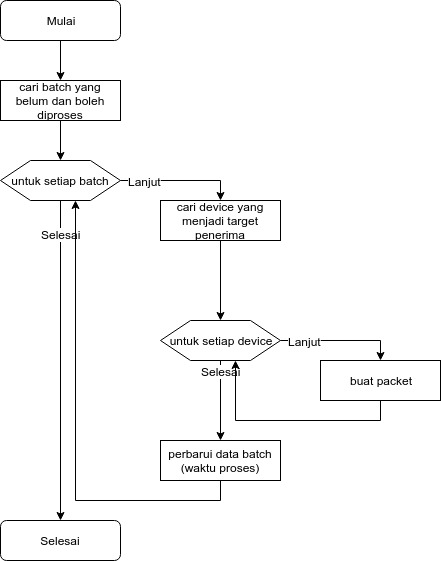
\includegraphics[width=1\textwidth]{bab3/figures/flowchart_pembuatan_packet.jpg}
    \caption{Diagram Alir Proses Pembuatan \textit{Packet}}
    \label{flowchart_pembuatan_packet}
\end{figure}

\subsubsection{Proses Menambahkan Packet ke Antrian}
\par Proses ini bertujuan untuk mengantrikan \textit{packet} yang sudah waktunya untuk dikirim.
Antrian \textit{packet} dibagi berdasarkan jenis perangkat penerima notifikasi (Android, Web, atau iOS). Proses pengantrian dapat dilihat di diagram alir pada gambar~\ref{flowchart_menambahkan_packet_ke_antrian}.
\begin{figure}[H]
    \centering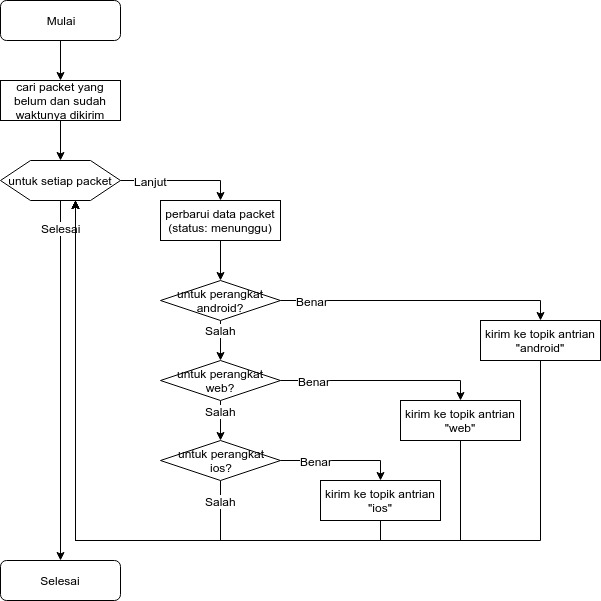
\includegraphics[width=1\textwidth]{bab3/figures/flowchart_menambahkan_packet_ke_antrian.jpg}
    \caption{Diagram Alir Proses Menambahkan \textit{Packet} ke Antrian}
    \label{flowchart_menambahkan_packet_ke_antrian}
\end{figure}

\subsubsection{Proses Pengiriman Packet ke APNs}
\par Proses ini bertujuan untuk mengirimkan \textit{packet} yang ada di antrian topik "ios" ke perangkat pengguna yang berbasis iOS lewat layanan APNs. Proses pengiriman \textit{packet} dapat dilihat di diagram alir pada
gambar~\ref{flowchart_pengiriman_packet_ke_apns}.
\begin{figure}[H]
    \centering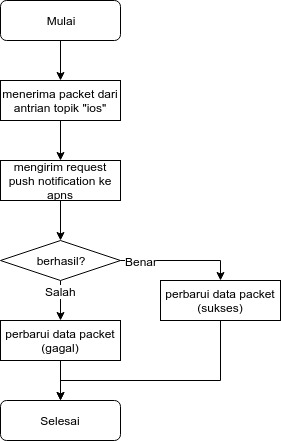
\includegraphics[width=0.8\textwidth]{bab3/figures/flowchart_pengiriman_packet_ke_apns.jpg}
    \caption{Diagram Alir Proses Pengiriman \textit{Packet} ke APNs}
    \label{flowchart_pengiriman_packet_ke_apns}
\end{figure}

\subsubsection{Proses Pengiriman Packet ke FCM}
\par Proses ini bertujuan untuk mengirimkan \textit{packet} yang ada di antrian topik "android" dan "web" ke perangkat pengguna yang berbasis Android atau Web lewat layanan FCM. Proses pengiriman \textit{packet} dapat dilihat di diagram alir pada gambar~\ref{flowchart_pengiriman_packet_ke_fcm}.
\begin{figure}[H]
    \centering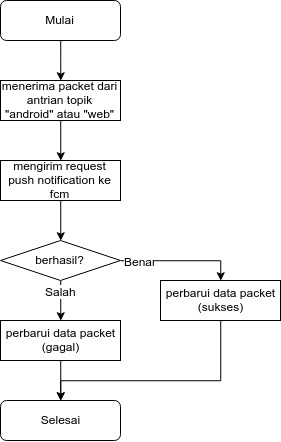
\includegraphics[width=0.8\textwidth]{bab3/figures/flowchart_pengiriman_packet_ke_fcm.jpg}
    \caption{Diagram Alir Proses Pengiriman \textit{Packet} ke FCM}
    \label{flowchart_pengiriman_packet_ke_fcm}
\end{figure}
